%package list
\documentclass{article}
\usepackage[top=3cm, bottom=3cm, outer=3cm, inner=3cm]{geometry}
\usepackage{multicol}
\usepackage{graphicx}
\usepackage{url}
%\usepackage{cite}
\usepackage{hyperref}
\usepackage{array}
%\usepackage{multicol}
\newcolumntype{x}[1]{>{\centering\arraybackslash\hspace{0pt}}p{#1}}
\usepackage{natbib}
\usepackage{pdfpages}
\usepackage{multirow}
\usepackage[normalem]{ulem}
\useunder{\uline}{\ul}{}
\usepackage{svg}
\usepackage{xcolor}
\usepackage{listings}

\lstdefinestyle{ascii-tree}{
    literate={├}{|}1 {─}{--}1 {└}{+}1 
  }
\lstset{basicstyle=\ttfamily,
  showstringspaces=false,
  commentstyle=\color{red},
  keywordstyle=\color{blue}
}
%\usepackage{booktabs}
\usepackage{caption}
\usepackage{subcaption}
\usepackage{float}
\usepackage{array}

\newcolumntype{M}[1]{>{\centering\arraybackslash}m{#1}}
\newcolumntype{N}{@{}m{0pt}@{}}


%%%%%%%%%%%%%%%%%%%%%%%%%%%%%%%%%%%%%%%%%%%%%%%%%%%%%%%%%%%%%%%%%%%%%%%%%%%%
%%%%%%%%%%%%%%%%%%%%%%%%%%%%%%%%%%%%%%%%%%%%%%%%%%%%%%%%%%%%%%%%%%%%%%%%%%%%
\newcommand{\itemEmail}{jgordillome@unsa.edu.pe}
\newcommand{\itemStudent}{Jose Alonzo Gordillo Mendoza}
\newcommand{\itemCourse}{Programación Web 2}
\newcommand{\itemCourseCode}{20220577}
\newcommand{\itemSemester}{III}
\newcommand{\itemUniversity}{Universidad Nacional de San Agustín de Arequipa}
\newcommand{\itemFaculty}{Facultad de Ingeniería de Producción y Servicios}
\newcommand{\itemDepartment}{Departamento Académico de Ingeniería de Sistemas e Informática}
\newcommand{\itemSchool}{Escuela Profesional de Ingeniería de Sistemas}
\newcommand{\itemAcademic}{2023 - A}
\newcommand{\itemInput}{Del 29 de Junio 2023}
\newcommand{\itemOutput}{Al 14 Julio 2023}
\newcommand{\itemPracticeNumber}{07}
\newcommand{\itemTheme}{Python - Django}
%%%%%%%%%%%%%%%%%%%%%%%%%%%%%%%%%%%%%%%%%%%%%%%%%%%%%%%%%%%%%%%%%%%%%%%%%%%%
%%%%%%%%%%%%%%%%%%%%%%%%%%%%%%%%%%%%%%%%%%%%%%%%%%%%%%%%%%%%%%%%%%%%%%%%%%%%

\usepackage[english,spanish]{babel}
\usepackage[utf8]{inputenc}
\AtBeginDocument{\selectlanguage{spanish}}
\renewcommand{\figurename}{Figura}
\renewcommand{\refname}{Referencias}
\renewcommand{\tablename}{Tabla} %esto no funciona cuando se usa babel
\AtBeginDocument{%
	\renewcommand\tablename{Tabla}
}

\usepackage{fancyhdr}
\pagestyle{fancy}
\fancyhf{}
\setlength{\headheight}{30pt}
\renewcommand{\headrulewidth}{1pt}
\renewcommand{\footrulewidth}{1pt}
\fancyhead[L]{\raisebox{-0.2\height}{
\includegraphics[width=3cm]{img/logo_episunsa.png}}}
\fancyhead[C]{\fontsize{7}{7}\selectfont	\itemUniversity \\ \itemFaculty \\ \itemDepartment \\ \itemSchool \\ \textbf{\itemCourse}}
\fancyhead[R]{\raisebox{-0.2\height}{
\includegraphics[width=1.2cm]{img/logo_abet}}}
\fancyfoot[L]{Estudiante Jose Gordillo Mendoza}
\fancyfoot[C]{\itemCourse}
\fancyfoot[R]{Página \thepage}

% para el codigo fuente
\usepackage{listings}
\usepackage{color, colortbl}
\definecolor{dkgreen}{rgb}{0,0.6,0}
\definecolor{gray}{rgb}{0.5,0.5,0.5}
\definecolor{mauve}{rgb}{0.58,0,0.82}
\definecolor{codebackground}{rgb}{0.95, 0.95, 0.92}
\definecolor{tablebackground}{rgb}{0.8, 0, 0}

\lstset{frame=tb,
	language=bash,
	aboveskip=3mm,
	belowskip=3mm,
	showstringspaces=false,
	columns=flexible,
	basicstyle={\small\ttfamily},
	numbers=none,
	numberstyle=\tiny\color{gray},
	keywordstyle=\color{blue},
	commentstyle=\color{dkgreen},
	stringstyle=\color{mauve},
	breaklines=true,
	breakatwhitespace=true,
	tabsize=3,
	backgroundcolor= \color{codebackground},
}

\begin{document}
	
	\vspace*{10px}
	
	\begin{center}	
		\fontsize{17}{17} \textbf{ Informe de Laboratorio \itemPracticeNumber}
	\end{center}
	\centerline{\textbf{\Large Tema: \itemTheme}}
	%\vspace*{0.5cm}	

	\begin{flushright}
		\begin{tabular}{|M{2.5cm}|N|}
			\hline 
			\rowcolor{tablebackground}
			\color{white} \textbf{Nota}  \\
			\hline 
			     \\[30pt]
			\hline 			
		\end{tabular}
	\end{flushright}	

	\begin{table}[H]
		\begin{tabular}{|x{4.7cm}|x{4.8cm}|x{4.8cm}|}
			\hline 
			\rowcolor{tablebackground}
			\color{white} \textbf{Estudiante} & \color{white}\textbf{Escuela}  & \color{white}\textbf{Asignatura}   \\
			\hline 
			{\itemStudent \par \itemEmail} & \itemSchool & {\itemCourse \par Semestre: \itemSemester \par Código: \itemCourseCode}     \\
			\hline 			
		\end{tabular}
	\end{table}		
	
	\begin{table}[H]
		\begin{tabular}{|x{4.7cm}|x{4.8cm}|x{4.8cm}|}
			\hline 
			\rowcolor{tablebackground}
			\color{white}\textbf{Laboratorio} & \color{white}\textbf{Tema}  & \color{white}\textbf{Duración}   \\
			\hline 
			\itemPracticeNumber & \itemTheme & 04 horas   \\
			\hline 
		\end{tabular}
	\end{table}
	
	\begin{table}[H]
		\begin{tabular}{|x{4.7cm}|x{4.8cm}|x{4.8cm}|}
			\hline 
			\rowcolor{tablebackground}
			\color{white}\textbf{Semestre académico} & \color{white}\textbf{Fecha de inicio}  & \color{white}\textbf{Fecha de entrega}   \\
			\hline 
			\itemAcademic & \itemInput &  \itemOutput  \\
			\hline 
		\end{tabular}
	\end{table}
	
	\section{Tarea}
	\begin{itemize}		
		\item Recreacion de los videos proporcionados en el aula virtual sobre relaciones one to many y many to many, asi como la generacion de pdf's y el envio de emails.
	\end{itemize}
        \begin{figure}[H]
		\centering
		
\includegraphics[width=0.25\textwidth,keepaspectratio]{img/django.png}
	\end{figure}

	\section{URL de Repositorio Github}
	\begin{itemize}
		\item URL para el laboratorio 07 en el Repositorio GitHub.
		\item \url{https://github.com/JoseGordilloMendoza/LAB07.git}
	\end{itemize}
	
	\section{Ejercicios}
 
        \subsection{Estructura de laboratorio 07}
	\begin{itemize}	
		\item La distribucion de archivos sera la siguiente (teniendo en cuenta los archivos mas importantes, por ejemplo las aplicaciones):
	\end{itemize}
	
\begin{lstlisting}[style=ascii-tree]
lab07/
    ├──lab07relations/
        ├── modelExa
             ├── __pycache__
             ├── migrations
             ├── __init__.py
             ├── admin.py
             ├── apps.py
             ├── models.py
             ├── tests.py
             ├── views.py
        ├── lab07relations 
             ├── __pycache__
             ├── migrations
             ├── __init__.py
             ├── asgi.py
             ├── settings.py
             ├── manage.py
             ├── urls.py
             ├── wsgi.py
        ├── db.sqlite3 
        ├── manage.py
        
    ├──lab07emails_pdf/
        ├── emails
             ├── emails
                 ├── __pycache__
                 ├── __init__.py
                 ├── asgi.py
                 ├── settings.py
                 ├── urls.py
                 ├── wsgi.py
             ├── send
                 ├── __pycache__
                 ├── migrations
                 ├── templates
                 ├── __init__.py
                 ├── admin.py
                 ├── models.py
                 ├── apps.py
                 ├── tests.py
                 ├── urls.py
                 ├── views.py
             ├── db.sqlite3
             ├── manage.py
        ├── pdfs
            ├── pdfs
                ├── __pycache__
                ├── __init__.py
                ├── asgi.py
                ├── settings.py
                ├── urls.py
                ├── wsgi.py
            ├── pdf
                ├── __pycache__
                ├── migrations
                ├── templates
                ├── __init__.py
                ├── admin.py
                ├── apps.py  
                ├── models.py
                ├── tests.py
                ├── utils.py
                ├── views.py
            ├── db.sqlite3
            ├── manage.py

\end{lstlisting}  
 
	\subsection{Relaciones One to many - Many to Many}
		\item En primer lugar veamos lo mas resaltante de modelsExa/apps.py:\newline\newline
        
	\begin{lstlisting}[language=bash,caption={Analizando modelsExa/apps.py}][H]
     from django.apps import AppConfig

    class ModelsexaConfig(AppConfig):
        default_auto_field = 'django.db.models.BigAutoField'
        name = 'modelsExa'
	\end{lstlisting}
         Este archivo de configuración de la aplicación ModelsexaConfig establece la configuración específica para la aplicación llamada 'modelsExa', incluyendo la configuración del campo de clave primaria automática. 
                  

        \begin{lstlisting}[language=bash,caption={models.py del proyecto}][H]
         from django.db import models
    
            class Simple(models.Model):
                text = models.CharField(max_length=10)
                number = models.IntegerField(null=True)
                url = models.URLField(default="www.example.com")
            
                def __str__(self):
                    return self.url
            class DateExample(models.Model):
                the_date = models.DateTimeField
            
            class NullExample(models.Model):
                col = models.CharField(max_length=10, blank=True, null=True)
            
            class Language(models.Model):
                name = models.CharField(max_length=10)
            
                def __str__(self):
                    return self.name
            
            class Framework(models.Model):
                name = models.CharField(max_length=10)
                language = models.ForeignKey(Language, on_delete=models.CASCADE)
            
                def __str__(self):
                    return self.name
                
            class Movie(models.Model):
                name = models.CharField(max_length=10)
            
                def __str__(self):
                    return self.name
            
            class Character(models.Model):
                name = models.CharField(max_length=10)
                movies = models.ManyToManyField(Movie)
            
                def __str__(self):
                 return self.name
	\end{lstlisting}
        Estas clases de modelos definen las estructuras y relaciones de base de datos para diferentes entidades, como "Simple", "DateExample", "NullExample", "Language", "Framework", "Movie" y "Character". Cada clase de modelo se mapea a una tabla en la base de datos y los campos de los modelos se traducen en columnas en esas tablas. Las relaciones entre los modelos se establecen mediante campos como ForeignKey y ManyToManyField.
        \begin{itemize}
            \item lab07\_one\_to\_many /modelsExample
        \end{itemize}
        \begin{lstlisting}[language=bash,caption={asgi.py}][H]
        import os

        from django.core.asgi import get_asgi_application
        
        os.environ.setdefault('DJANGO_SETTINGS_MODULE', 'modelsExample.settings')
        
        application = get_asgi_application()

	\end{lstlisting}
   Este código configura el entorno y obtiene una instancia del servidor de aplicaciones ASGI para la aplicación Django definida en el módulo de configuración 'modelsExample.settings'. Esta instancia del servidor de aplicaciones se utiliza para manejar las solicitudes y respuestas HTTP de la aplicación cuando se ejecuta utilizando un servidor compatible con ASGI.
    
        \begin{lstlisting}[language=bash,caption={settings.py}][H]
            INSTALLED_APPS = [
                'django.contrib.admin',
                'django.contrib.auth',
                'django.contrib.contenttypes',
                'django.contrib.sessions',
                'django.contrib.messages',
                'django.contrib.staticfiles',
                'modelsExa',
            ]
	\end{lstlisting}
    Al incluir 'modelsExa' en INSTALLED\_APPS, me aseguro de que Django reconozca y utilice la aplicación personalizada en el proyecto. Esto permite que los modelos y otros componentes de la aplicación estén disponibles y se integren con el resto del sistema de Django.
        
        \begin{lstlisting}[language=bash,caption={wsgi.py}][H] 
           import os

            from django.core.wsgi import get_wsgi_application
            
            os.environ.setdefault('DJANGO_SETTINGS_MODULE', 'modelsExample.settings')
            
            application = get_wsgi_application()
            
	\end{lstlisting}
    Este código configura el entorno y obtiene una instancia del servidor de aplicaciones WSGI para la aplicación Django definida en el módulo de configuración 'modelsExample.settings'.

        
        \subsection{Generaciónn de pdf}
        \begin{itemize}
            \item Analizando la configuracion del proyecto
        \end{itemize}
        \begin{lstlisting}[language=bash,caption={Archivo settings.py}][H]
            INSTALLED_APPS = [
                'django.contrib.admin',
                'django.contrib.auth',
                'django.contrib.contenttypes',
                'django.contrib.sessions',
                'django.contrib.messages',
                'django.contrib.staticfiles',
                'pdf',
            ]
	\end{lstlisting}
        En este fragmento vemos lo mas resaltante de settings.py, pues tenemos una aplicacion llamada pdf de la cual obtendremos la principal logica de nuestra pagina.
        \newline
        
        \begin{itemize}
            \item Analizando las url del proyecto
        \end{itemize}
        \begin{lstlisting}[language=bash,caption={Archivo urls.py}][H]
            from django.contrib import admin
            from django.urls import path
            from pdf.views import GeneratePdf
            
            urlpatterns = [
                path('admin/', admin.site.urls),
                path('pdf/',GeneratePdf.as_view(), name='PDF'),
            ]
	\end{lstlisting}
        Como vemos tendremos una url "pdf" que sera la que imprima un pdf como tal haciendo uso de una view; esto teniendo en cuenta que importaremos las urls de la aplicacion pdf.

        \begin{itemize}
            \item En la app pdf, analizaremos el archivo utils.py
        \end{itemize}
        \begin{lstlisting}[language=bash,caption={Archivo pdf/utils.py}][H]
            from io import BytesIO
            from django.http import HttpResponse
            from django.template.loader import get_template
            
            from xhtml2pdf import pisa
            
            def render_to_pdf(template_src, context_dict={}):
                template = get_template(template_src)
                html  = template.render(context_dict)
                result = BytesIO()
                pdf = pisa.pisaDocument(BytesIO(html.encode("ISO-8859-1")), result)
                if not pdf.err:
                    return HttpResponse(result.getvalue(), content_type='application/pdf')
                return None
	\end{lstlisting}
        En esta función toma una plantilla HTML, la renderiza con los datos del contexto y la convierte en un archivo PDF utilizando xhtml2pdf. Luego, devuelve una respuesta HTTP que contiene el PDF generado.
        Hay que saber que utils.py es un archivo comúnmente utilizado en proyectos Django para almacenar funciones y clases de utilidad que se utilizan en varias partes del proyecto. Es una práctica común separar estas funciones y clases en un archivo aparte para mantener un código más organizado y modular. \newline

         \begin{itemize}
            \item Vistas de la app
        \end{itemize}
        \begin{lstlisting}[language=bash,caption={Archivo pdf/views.py}][H]
            from django.shortcuts import render

            from django.http import HttpResponse
            from django.template.loader import get_template
            from django.views.generic import View
            
            from .utils import render_to_pdf #created in step 4
            
            class GeneratePdf(View):
                def get(self, request, *args, **kwargs):
                    template = get_template('invoice.html')
                    context = {
                         'today': "Today", 
                         'amount': 1339.99,
                        'customer_name': 'Cooper Mann',
                        'invoice_id': 1233434,
                    }
                    html = template.render(context)
                    pdf = render_to_pdf('invoice.html',context)
                    if pdf:
                        response = HttpResponse(pdf, content_type='application/pdf')
                        filename = "Invoice_%s.pdf"%("12341231")
                        content = "inline; filename='%s'"%(filename)
                        download = request.GET.get("download")
                        if download:
                            content = "attachment; filename='%s'" %(filename)
                        response['Content-Disposition']=content
                        return response  
            
                    return HttpResponse("Not Found")
	\end{lstlisting}
        Esta vista basada en clase permite generar y devolver un archivo PDF a partir de una plantilla HTML cuando se realiza una solicitud HTTP GET a la vista. El archivo PDF puede ser descargado o mostrado en el navegador según los parámetros proporcionados en la URL de la solicitud. A resaltar que se importa la función render\_to\_pdf desde un archivo utils.py, que se supone que contiene una función personalizada para generar un archivo PDF a partir de una plantilla HTML.\newline

         \begin{itemize}
            \item HTML de la app
        \end{itemize}
        \begin{lstlisting}[language=bash,caption={Archivo pdf/templates/invoice.html}][H]
            <!DOCTYPE HTML PUBLIC "-//W3C//DTD HTML 4.01 Transitional//EN" "http://www.w3.org/TR/html4/loose.dtd">
            <html>
                <head>
                    <title>Title</title>
                    <style type="text/css">
                        body {
                            font-weight: 200;
                            font-size: 14px;
                        }
                        .header {
                            font-size: 20px;
                            font-weight: 100;
                            text-align: center;
                            color: #007cae;
                        }
                        .title {
                            font-size: 22px;
                            font-weight: 100;
                           /* text-align: right;*/
                           padding: 10px 20px 0px 20px;  
                        }
                        .title span {
                            color: #007cae;
                        }
                        .details {
                            padding: 10px 20px 0px 20px;
                            text-align: left !important;
                            /*margin-left: 40%;*/
                        }
                        .hrItem {
                            border: none;
                            height: 1px;
                            /* Set the hr color */
                            color: #333; /* old IE */
                            background-color: #aca0a0; /* Modern Browsers */
                        }
                    </style>
                </head>
                <body>
                    <div class='wrapper'>
                        <div class='header'>
                            <p class='title'>Invoice # </p>
                        </div>
                    <div>
                    <div class='details'>
                        Bill to: {{customer_name}}<br/>
                        Amount:  {{amount}}<br/>
                        Date: {{today}}
                        <hr class='hrItem' />
                    </div>
                </div>
                </body>
            </html>
	\end{lstlisting}
        Esta plantilla HTML define la estructura y los estilos básicos para generar un documento con un encabezado, detalles y una línea horizontal para separar secciones. Los datos del cliente, el monto y la fecha se insertarán en los lugares correspondientes utilizando variables del contexto cuando se renderice la plantilla.\newline

        
        \begin{itemize}
            \item Demostracion en navegador\newline
            
        \end{itemize}
        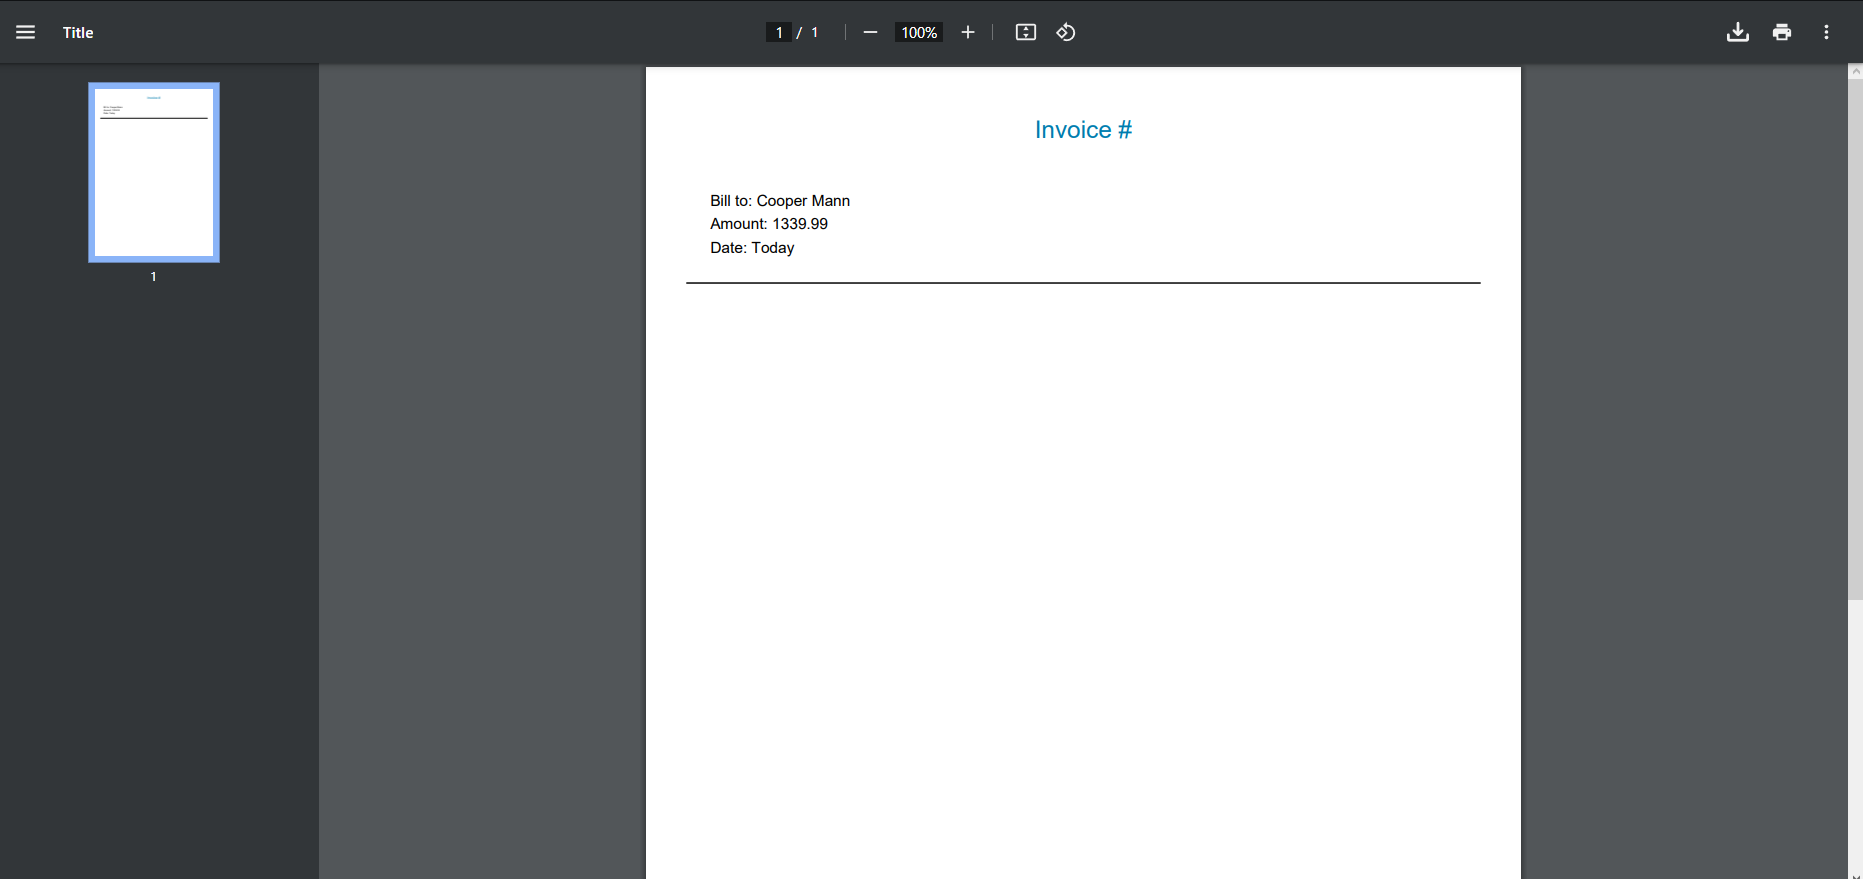
\includegraphics[width=16cm]{img/PDF DEMOSTRACION IMG.png}
        \newline En la captura vemos el pdf que se genera al entrar a la url .../pdf, cabe resaltar que la direccion predeterminada que se suele usar .../ no esta definida, por lo que el pdf se generera en la de pdf.
        
        \subsection{Envio de email}
        
        \begin{itemize}
            \item Analizando la configuracion del proyecto
        \end{itemize}
        \begin{lstlisting}[language=bash,caption={Archivo settings.py}][H]
            INSTALLED_APPS = [
                'django.contrib.admin',
                'django.contrib.auth',
                'django.contrib.contenttypes',
                'django.contrib.sessions',
                'django.contrib.messages',
                'django.contrib.staticfiles',
                'send',
                
            ]

            ...

            EMAIL_HOST = 'smtp.gmail.com'
            EMAIL_PORT = 587
            
            EMAIL_HOST_USER ='sjbalonzo201c@gmail.com'
            EMAIL_HOST_PASSWORD = 'ifhkdehiucgqrcmg'
            EMAIL_USE_TLS = True
            EMAIL_USE_SSL = False
	\end{lstlisting}
        En este fragmento vemos lo mas resaltante de settings.py, pues tenemos una aplicacion llamada send de la cual obtendremos la principal logica de nuestra pagina.
        Por otra parte configuramos lo concerniente al correo, estas configuraciones se utilizan en Django para enviar correos electrónicos a través del servidor SMTP de Gmail. Asegúrate de proporcionar correctamente tu dirección de correo electrónico y contraseña en EMAIL\_HOST\_USER y EMAIL\_HOST\_PASSWORD, respectivamente, para permitir que Django se autentique en el servidor SMTP de Gmail y envíe correos electrónicos desde esa cuenta.
        Es muy importante mencionar que el password se configura en la cuenta de gmail habilitando/generando una "contraseña de aplicaciones" pues con la contraseña usual nos saltara un error.
        \newline

        \begin{itemize}
            \item Analizando las url del proyecto
        \end{itemize}
        \begin{lstlisting}[language=bash,caption={Archivo urls.py}][H]
            from django.contrib import admin
            from django.urls import path, include
            
            urlpatterns = [
                path('admin/', admin.site.urls),
                path('', include('send.urls')),
            ]
	\end{lstlisting}
        Como vemos tendremos una url "" que sera la que envie un email como tal haciendo uso de una view; esto teniendo en cuenta que importaremos las urls de la aplicacion send, que es la que contiene la url original.

        
         \begin{itemize}
            \item En la app send, analizaremos el archivo urls.py
        \end{itemize}
        \begin{lstlisting}[language=bash,caption={Archivo send/urls.py}][H]
            from django.urls import path, include
            from . import views
            
            urlpatterns = [
            
                path('', views.index),
            ]
	\end{lstlisting}
        Esta configuración de URLs indica que cuando se acceda a la ruta principal del sitio, se ejecutará la vista index definida en el módulo views. Puedes agregar más objetos path a la lista urlpatterns para mapear otras rutas de URL a diferentes vistas en tu aplicación Django.\newline

        \begin{itemize}
            \item Analizaremos el archivo views.py
        \end{itemize}
        \begin{lstlisting}[language=bash,caption={Archivo send/views.py}][H]
            from django.shortcuts import render
            from django.core.mail import send_mail
            
            # Create your views here.
            def index(request):
                send_mail('EMAIL DESDE DJANGO',
                          'Probando envio de email desde DJANGO, hola :D',
                          'sjbalonzo201c@gmail.com',
                          ['jgordillome@unsa.edu.pe'],
                          fail_silently=False)
                return render(request, 'send/index.html')

	\end{lstlisting}
         Esta vista en Django envía un correo electrónico utilizando la función send\_mail y luego renderiza una plantilla HTML llamada 'send/index.html'. Podemos personalizar los detalles del correo electrónico, como el asunto, el cuerpo y las direcciones de los remitentes y destinatarios, según las necesidades.\newline

         \begin{itemize}
            \item Analizaremos el archivo templates/send/index.html
        \end{itemize}
        \begin{lstlisting}[language=bash,caption={Archivo send/templates/send/index.html}][H]
            <!DOCTYPE html>
            <html lang="en">
              
              <head>
                <title>Sent!</title>
              </head> 
              <body>
                <h1>sent an email!</h1>
              </body>
            
            </html>

	\end{lstlisting}
         Eesta plantilla HTML muestra un mensaje simple "sent an email!" en el cuerpo del documento. Usada para mostrar una confirmación de que se ha enviado correctamente un correo electrónico desde una aplicación Django, por ejemplo, después de llamar a la función send\_mail en una vista y redirigir a esta plantilla.\newline

        \begin{itemize}
            \item Demostracion en navegador\newline
            
        \end{itemize}
        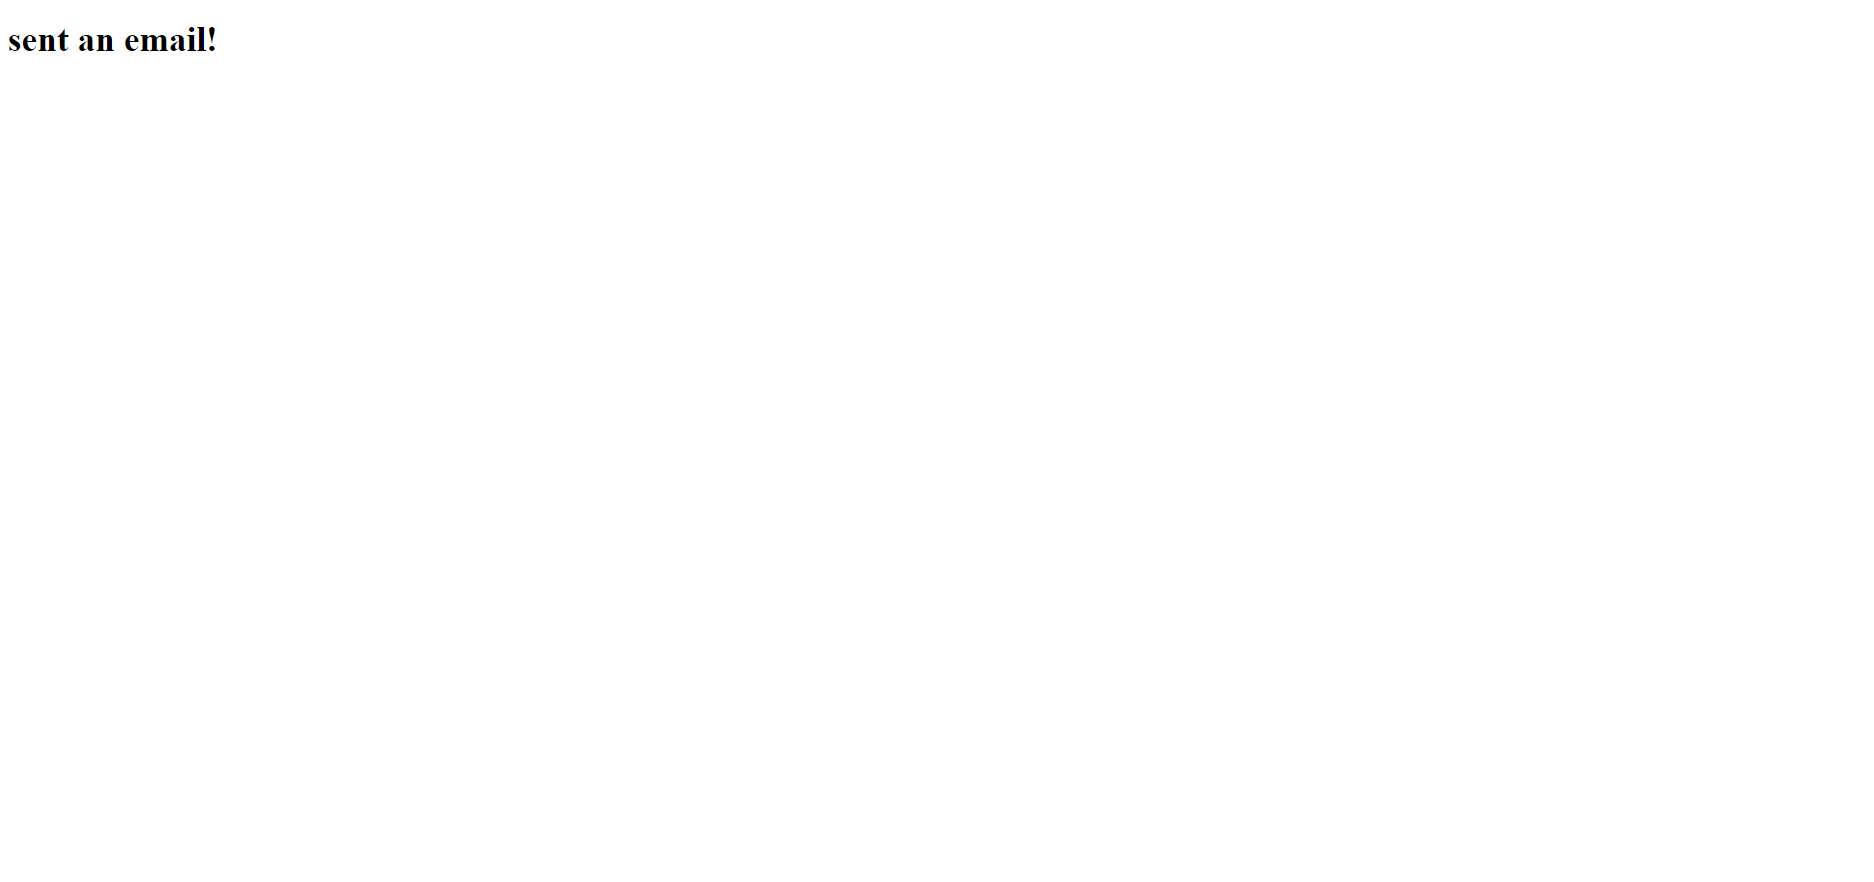
\includegraphics[width=16cm]{img/INDEX EMAIL.png}
        \newline En la captura vemos que la pagina mostrandonos un mensaje de que se envio el email; por tanto veamos como llega al correo especificado en la vista.

        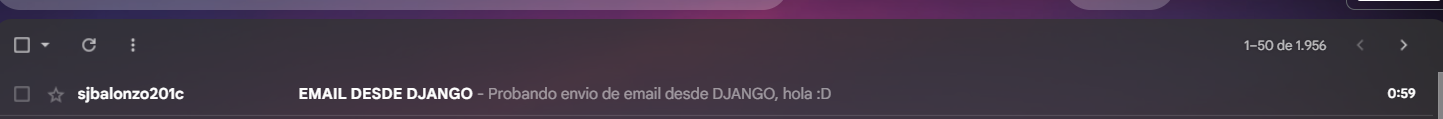
\includegraphics[width=16cm]{img/correo recibido.png}
        \newline Ahora vemos como nos ha llegado a nuestro correo.

        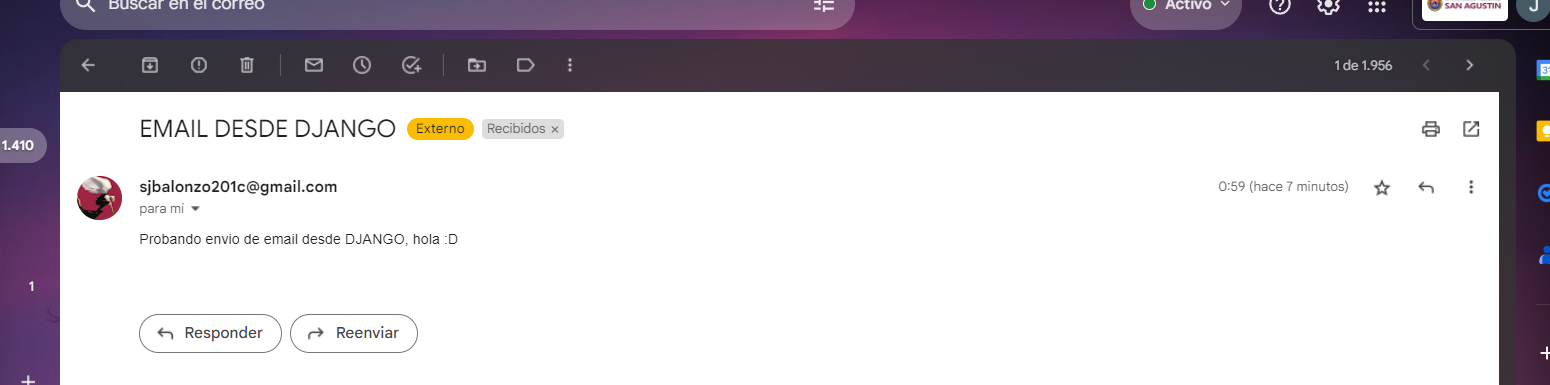
\includegraphics[width=16cm]{img/email recibido.png}
        \newline Como vemos nos muestra lo que especificamos anteriormente en nuestra view, es decir: asunto, mensaje, remitente y destinario.
        \newline
        \newline\newline 
        Link donde esta alojado el video (FlipGrid):\newline
        GRUPO:
        \url{https://flip.com/8a44775d}\newline
        VIDEO ESPECIFICO:
        \url{}
        
\section{Cuestionario}
	- Sin cuestionario -	
 \newpage
 \section{Conclusiones}
	\begin{itemize}
		\item Django proporciona un sólido sistema de relaciones que permite establecer vínculos entre diferentes modelos. Las relaciones "one-to-many" permiten establecer una conexión en la que un modelo está relacionado con varios modelos de otro tipo. Las relaciones "many-to-many" permiten una mayor flexibilidad, ya que un modelo puede estar vinculado a múltiples instancias de otro modelo y viceversa.
            \item En las relaciones "many-to-many", Django utiliza una tabla intermedia para almacenar los vínculos entre los modelos. Esta tabla contiene claves foráneas que apuntan a las instancias de los modelos relacionados. Por ejemplo, si tenemos un modelo de "Estudiante" y un modelo de "Curso", la tabla intermedia contendría claves foráneas que enlazarían estudiantes con cursos y viceversa.
            \item Una ventaja clave de utilizar relaciones en Django es la capacidad de acceder a los objetos relacionados a través de consultas. Por ejemplo, si tienes un modelo de "Autor" relacionado con varios modelos de "Libro", puedes acceder a los libros de un autor específico utilizando la relación definida en el modelo. Esto facilita la navegación entre modelos y la recuperación de datos relacionados.
            \item En las relaciones "many-to-many", Django utiliza una tabla intermedia para almacenar los vínculos entre los modelos. Esta tabla contiene claves foráneas que apuntan a las instancias de los modelos relacionados. Por ejemplo, si tenemos un modelo de "Estudiante" y un modelo de "Curso", la tabla intermedia contendría claves foráneas que enlazarían estudiantes con cursos y viceversa.
	\end{itemize}	
\clearpage

\section{Referencias}
\begin{itemize}	
    \item \url{https://www.w3schools.com/python/python_reference.asp}
    \item \url{https://docs.djangoproject.com/en/4.2/topics/email/}
    \item \url{https://www.scaler.com/topics/django/relationships-in-django-models/}
    \item \url{https://docs.djangoproject.com/en/4.2/howto/outputting-pdf/}
\end{itemize}	
	
%\clearpage
%\bibliographystyle{apalike}
%\bibliographystyle{IEEEtranN}
%\bibliography{bibliography}
			
\end{document}